\documentclass[12pt]{ucsddissertation}
% mathptmx is a Times Roman look-alike (don't use the times package)
% It isn't clear if Times is required. The OGS manual lists several
% "standard fonts" but never says they need to be used.
\usepackage{mathptmx}
\usepackage[NoDate]{currvita}
\usepackage{array}
\usepackage{tabularx}
\usepackage{booktabs}
\usepackage{ragged2e}
\usepackage{microtype}
\usepackage[breaklinks=true,pdfborder={0 0 0}]{hyperref}
\usepackage{graphicx}
\AtBeginDocument{%
	\settowidth\cvlabelwidth{\cvlabelfont 0000--0000}%
}

% OGS recommends increasing the margins slightly.
\increasemargins{.1in}

% These are just for testing/examples, delete them
\usepackage{trace}
%\usepackage{showframe} % This package was just to see page margins
\usepackage[english]{babel}
\usepackage{blindtext}
\overfullrule5pt
% ---

% Required information
\title{This is the Title of My Dissertation}
\author{My Full Legal Name}
\degree{My Degree Title}{Doctor of Philosophy/Doctor of Musical
Arts/\par Doctor of Education}
% Each member of the committee should be listed as Professor Foo Bar.
% If Professor is not the correct title for one, then titles should be
% omitted entirely.
\chair{Professor Eta Theta}
\cochair{Professor Gamma Delta} % Optional
% Your committee members (other than the chairs) must be in alphabetical order
\committee{Professor Lambda Kappa}
\committee{Professor Iota Mu}
\committee{Professor Epsilon Zeta}
\degreeyear{2023}

% Start the document
\begin{document}
% Begin with frontmatter and so forth
\frontmatter
\maketitle
\makecopyright
\makesignature
% Optional
\begin{dedication}
\setsinglespacing
\raggedright % It would be better to use \RaggedRight from ragged2e
\parindent0pt\parskip\baselineskip
In recognition of reading this manual before beginning to format the
doctoral dissertation or master's thesis; for following the
instructions written herein; for consulting with OGS Academic Affairs
Advisers; and for not relying on other completed manuscripts, this
manual is dedicated to all graduate students about to complete the
doctoral dissertation or master's thesis.

In recognition that this is my one chance to use whichever
justification, spacing, writing style, text size, and/or textfont that
I want to while still keeping my headings and margins consistent.
\end{dedication}
% Optional
\begin{epigraph}
\vskip0pt plus.5fil
\setsinglespacing
{\flushright
True ease in writing comes from art, not chance,\\
As those move easiest who have learn'd to dance.\\
'T is not enough to no harshness gives offence,---\\
The sound must seem an echo to the sense.

\vskip\baselineskip
\textit{Alexander Pope}\par}
\vfil
\begin{center}
You write with ease to show your breeding,\\
But easy writing's curst hard reading.

\vskip\baselineskip
\textit{Richard Brinsley Sheridan}
\end{center}
\vfil
\noindent Writing, at its best, is a lonely life. Organizations for
writers palliate the writer's loneliness, but I doubt if they improve
his writing. He grows in public stature as he sheds his loneliness and
often his work deteriorates. For he does his work alone and if he is a
good enough writer he must face eternity, or the lack of it, each day.

\vskip\baselineskip
\hskip0pt plus1fil\textit{Ernest Hemingway}\hskip0pt plus4fil\null

\vfil
\end{epigraph}

% Next comes the table of contents, list of figures, list of tables,
% etc. If you have code listings, you can use \listoflistings (or
% \lstlistoflistings) to have it be produced here as well. Same with
% \listofalgorithms.
\tableofcontents
\listoffigures
\listoftables

% Preface
\begin{preface}
Almost nothing is said in the manual about the preface. There is no
indication about how it is to be typeset. Given that, one is forced to
simply typeset it and hope it is accepted. It is, however, optional
and may be omitted.
\end{preface}

% Your fancy acks here. Keep in mind you need to ack each paper you
% use. See the examples here. In addition, each chapter ack needs to
% be repeated at the end of the relevant chapter.
\begin{acknowledgements}
I would like to acknowledge Professor Eta Theta for his support as the
chair of my committee. Through multiple drafts and many long nights,
his guidance has proved to be invaluable.

I would also like to acknowledge the ``Smith Clan'' of lab~28, without
whom my research would have no doubt taken fives times as long. It is
their support that helped me in an immeasureable way.

Chapter 2, in full, is a reprint of the material as it appears in
Numerical Grid Generational in Computational Fluid Mechanics~2009.
Smith, Laura; Smith, Jane~D., Pineridge Press,~2009. The dissertation
author was the primary investigator and author of this paper.

Chapter 3, in part, has been submitted for publication of the material
as it may appear in Education Mechanics,~2009, Smith, Laura; Smith,
Jane~D., Trailor Press,~2009. The dissertation author was the primary
investigator and author of this paper.

Chapter 5, in part is currently being prepared for submission for
publication of the material. Smith, Laura; Smith, Jane~D\@. The
dissertation author was the primary investigator and author of this
material.
\end{acknowledgements}

% Stupid vita goes next
\begin{vita}
\noindent
\begin{cv}{}
\begin{cvlist}{}
\item[1996] Bachelor of Arts, University of California, Berkeley
\item[1996--2000] U.S. Marines
\item[2000--2002] Teaching Assistant, Department of Mechanical
Engineering\\University of California, San Diego
\item[2002--2006] Research Assistant, University of California, San
Diego
\item[2010] Doctor of Philosophy, University of California, San Diego
\end{cvlist}
\end{cv}

% This puts in the PUBLICATIONS header. Note that it appears inside
% the vita environment. It is optional.
\publications
\noindent``Distributions of Control Points in a System for Analysis of Stress
Distribution'' IRE Transactions of the I.R.E\@. Professional Group on
Automatic Control, vol. AC-7, pp 272--289, September 2005

% This puts in the FIELDS OF STUDY. Also inside vita and also
% optional.
\fieldsofstudy
\noindent Major Field: Engineering (Specialization or Focused Studies)
\vskip\baselineskip
Studies in Applied Mathematics\par
Professors Alpha Beta and Gamma Delta
\vskip\baselineskip
Studies in Mechanices\par
Professors Epsilon Zeta and Eta Theta
\vskip\baselineskip
Studies in Electromagnetism\par
Professors Iota Kappa and Lambda Mu
\end{vita}

% Put your maximum 350 word abstract here.
\begin{dissertationabstract}
The Abstract begins here. The abstract is limited to 350 words for a
doctoral dissertation. It should consist of a short statement of the
problem, a brief explanation of the methods and procedures employed in
generating the data, and a condensed summary of the findings of the
study. The abstract may continute onto a second page if necessary. The
text of the abstract must be double spaced.
\end{dissertationabstract}

% This is where the main body of your dissertation goes!
\mainmatter


\chapter{Introduction}
\section{Motivation}
Robotic manipulation is a fundamental field in robotics. Over the last two decades, robotics arms have become core tools in many industries such as car manufacturing, minimally invasive surgical operations and precision assembly of electronics. However, open-world manipulation tasks still remain a largely unsolved problem\cite{Tedrake_2023}.  An example of such a task is shown in \ref{fig:exampleTask}. One of the main reasons current systems' performance are unsatisfactory at such tasks is that we expect robots to achieve human level performance in such tasks while current robots are ill-equipped to deal with such tasks. Robotic manipulators don't have the same amount of computing resource, sensing capabilities as well as the suitable hardware to succeed in manipulation tasks \cite{Wang_Liu_Zhang_Lu_2020} \cite{Xue_Ju_Xiang_Chen_Liu_2017}. For instance, in pick-and-place tasks, humans easily manipulate unseen objects in complex environments in a stable and robust manner. However, most robots use parallel gripper for their low cost and ease of control. As a result, such grippers provide much less points of contact compared to the human hand, thus limiting the amount of stable grasp poses. This makes stable and robust manipulation challenging. This deficit in hardware calls for creative algorithms tailored for current robotic hardware that both ensures performance and robustness in open-world environments.

\section{Contributions}
The main contribution of this thesis is a learning and physically based grasp analyzer that can differentiate between stable lifting and stable sliding poses. The grasp analyzer consists of three parts: a learning-based 6-DoF grasp proposer (pre-trained model, not novel), a learning-based center of mass estimator, and a physics based grasp classifier that determines the quality of each proposed grasp. This grasp analyzer is intended to use with a multi-modal planner. Together, the system enables stable object manipulation in table-top environments even in cluttered environments containing objects with complicated shapes.

\begin{figure}
	\centering
	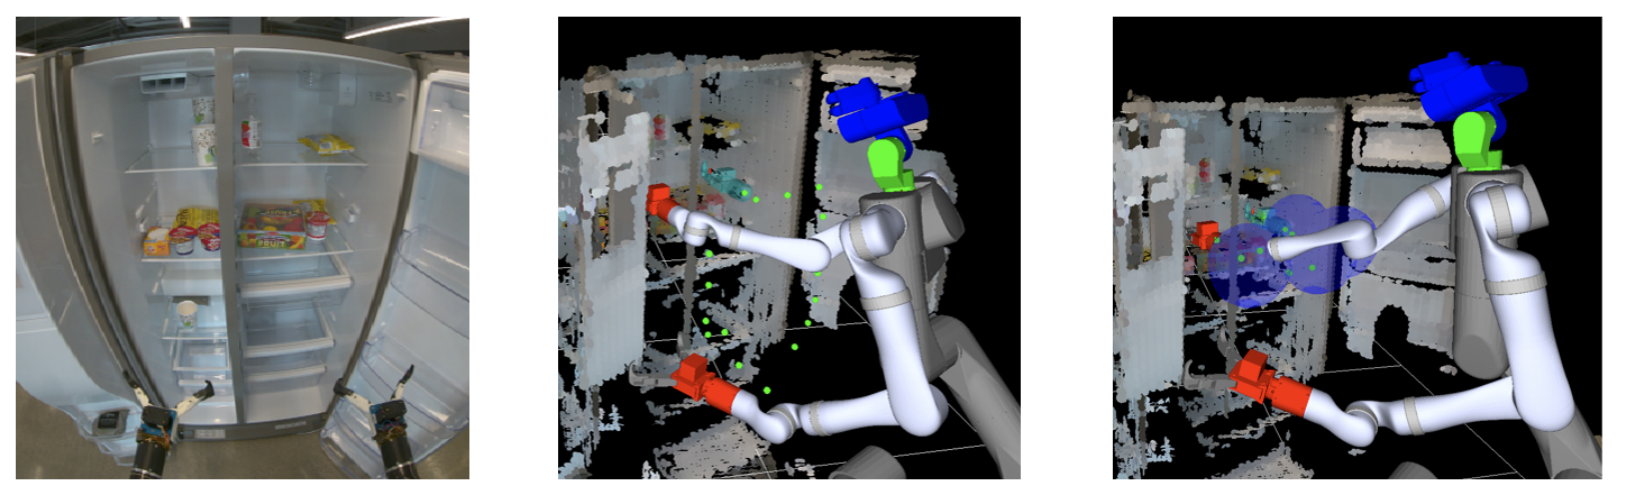
\includegraphics[width=\linewidth]{figures/exampleTask.png}
	\caption[An example of a pick-and-place task]{An example of a robotic manipulation task in a home environment. The green dots signify the planned path for the end effecter to take. \cite{Cheng_Shankar_Burdick_2020}}
	\label{fig:exampleTask}
\end{figure}

\chapter{Background}
This section provides background for each of the individual components of the grasp analyzer.

\section{Center of Mass Estimation}
Humans have an inert ability to estimate the center of mass of common objects through vision alone. This ability enables us to manipulate objects stably as we will minimize the torque generated by a grasp. Conversely, center of mass estimation has also been an important part in the classical (non-learning) approach to grasping \cite{Kanoulas_Lee_Caldwell_Tsagarakis_2018}, \cite{Yong_Yu_Fukuda_Tsujio_1999}. \cite{Yong_Yu_Fukuda_Tsujio_1999} proposed a method that uses the gravity equi-effect plane of an object under external force to determine the center of mass of a polyhedron. However, this method requires the robot to tip the object repeated, which may not be feasible in cluttered environments. Moreover, since a lot of common objects are not polyhedrons, the application and accuracy of the method may be limited. \cite{Kanoulas_Lee_Caldwell_Tsagarakis_2018} formulated the process of grasping and finding the center of mass of the object as a reinforcement learning problem. An initial estimate of the CoM (center of mass) is found by finding the centroid of a segmented object's point cloud. Using this CoM, the grasp with the lowest expected torque is executed by the robot and the actual grasp torque is measured by force sensors. This data is then used to re-evaluate the CoM, repeating the procedure until a satisfactory low-torque grasp has been found. This method could lead to irrecoverable failures as a grasp must be executed to calibrate the center of mass found. More importantly, the centroid of a point cloud is not a reliable estimator for center of mass as the full point cloud of an object is usually not attainable in open-world environments. The centroid of partial point cloud may be misleading, causing slippage during grasp.

\section{Grasp Pose Proposer}
Due to the limited contact points provided by a parallel gripper, finding a suitable grasp pose becomes a challenging problem. In recent years, machine learning has a become popular approach for grasp proposers \cite{ten_Pas_Gualtieri_Saenko_Platt_2017}, \cite{Mousavian_Eppner_Fox_2019}, \cite{Sundermeyer_Mousavian_Triebel_Fox_2021}. These learning-based methods are able to generate a set of 6-DoF grasp poses for parallel grippers from raw point cloud data. \cite{ten_Pas_Gualtieri_Saenko_Platt_2017} proposed a CNN that is trained using artificial data. The data consists of sampled grasp poses that are labeled as good and bad grasp poses. \cite{Mousavian_Eppner_Fox_2019} proposed a two-part framework where a VAE is trained to sample poses with a point cloud input and an evaluation module is trained to detect and refine the proposed grasps. Contact-GraspNet\cite{Sundermeyer_Mousavian_Triebel_Fox_2021} simplified the representation of grasp poses from 6-DoF to 4-DoF to improve model training. It also used the ACRONYM \cite{Eppner_Mousavian_Fox_2021} dataset, a large simulation-based dataset with a vast amount of different object types. Contact-GraspNet was able to achieve state-of-the-art performance on many benchmarks while being lightweight. It consisted of only one network with a Pointnet++ \cite{Qi2017PointNetDH} encoder backbone and returned directly usable grasp poses. However, since ACRONYM's grasp poses are classified under a zero-gravity environment, the grasp poses generated by Contact-GraspNet do not consider instabilities such as rotation and slippage when the objects' pose change relative to gravity. This leads to the model proposing grasp poses that can be maintained but is unstable. This is shown in \ref{fig:exampleGrasps}.

\begin{figure}
	\centering
	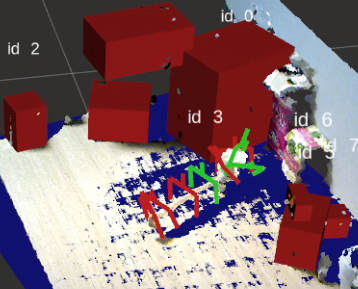
\includegraphics[width=250pt]{figures/grasps.png}
	\caption[Sample grasps from Contact-GraspNet]{Some grasp poses generated by Contact-GraspNet. The red grasp poses are not stable if the object is being lifted, while the green ones are stable lifting grasp poses. The poses are classified by the algorithm proposed.}
	\label{fig:exampleGrasps}
\end{figure}

\section{Grasp Stability Analysis}
A grasp may fail in two possible ways: slippage or rotation. Slippage refers to the scenario when the contact friction between the gripper and the object is not sufficient to support the object's weight. Rotation refers to the the scenario when the static torque between the gripper and the object is not sufficient to balance out the object's gravitational torque. In general, current learning-based methods generates grasps that are immune to slippage. However, since point cloud data does not encode gravitational information, rotation slippage is a common appearance. Therefore, the primary concern of a grasp stability analyzer is the static torques exerted on the object by the gripper and the gravitational torque of the object.


\chapter{Methodology}
The grasp analyzer consists of a grasp proposer, a center of gravity (CoM) estimator, and a grasp classifier. The first two components are learning-based; the grasp classifier is a physics-based torque analyzer. For the grasp proposer, a pre-trained version of Contact-GraspNet \cite{Sundermeyer_Mousavian_Triebel_Fox_2021} is used. Contact-GraspNet is chosen for its simplicity as well as its state-of-the-art performance in tabletop scenarios. The CoM estimator and the grasp classifier will be discussed in more details in the following sections.

\begin{figure}
	\centering
	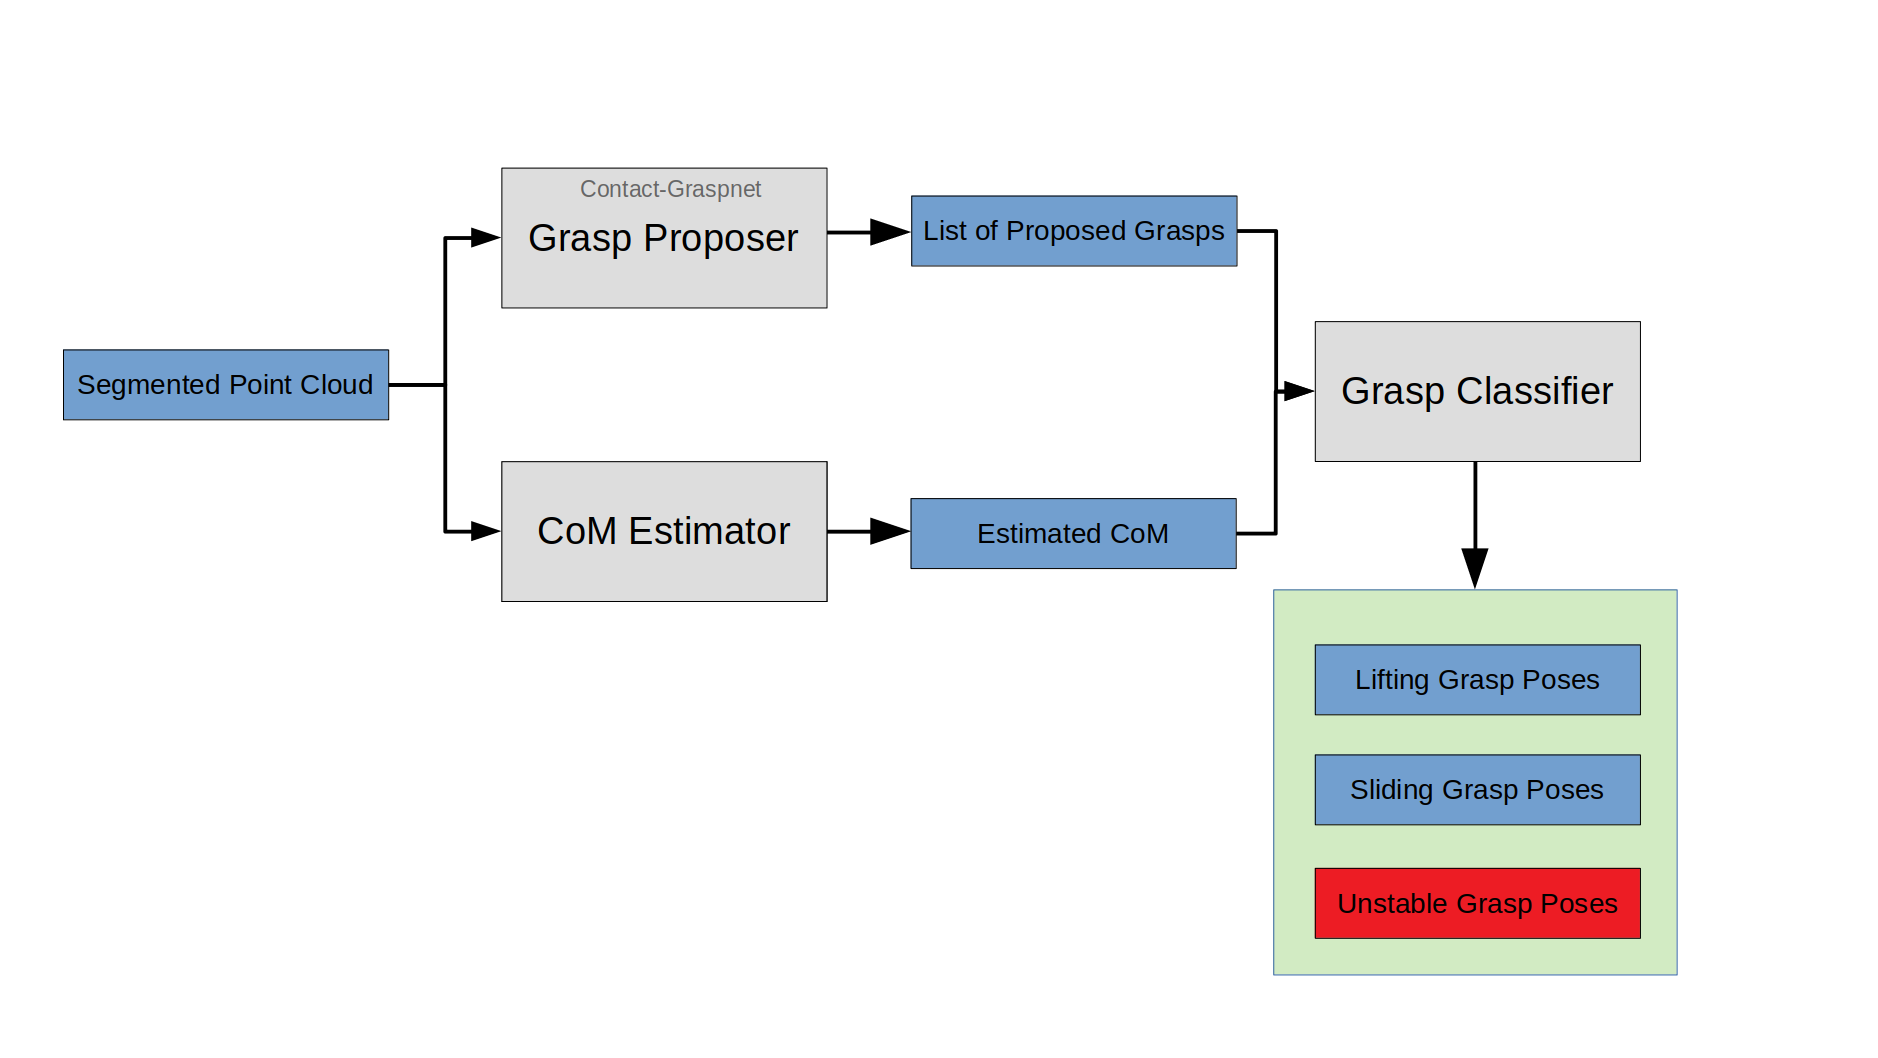
\includegraphics[width=\linewidth]{figures/overallPipeline.png}
	\caption[Overall Pipeline of the proposed grasp analyzer]{The overall pipeline of the grasp analyzer is shown here. The grasp proposer and the CoM estimator take segmented point cloud are input and output a list of proposed grasps and an estimated CoM. The two are then analyzed the the grasp classifier to determine which grasps are table lifting grasps, stable sliding grasps or neither. Note that a grasp can be both a stable lifting grasp and a stable sliding grasp.}
	\label{fig:overallPipeline}
\end{figure}

\section{Center of Mass Estimator}
\subsection{Architecture}
The architecture of the center of mass estimator is shown in \ref{fig:architecture}. Similar to Contact-GraspNet, the first part of the architecture utilizes a Pointnet++ feature extractor to create per-point features from segmented point cloud. This feature is then passed into three fully connected layers. Note that the fully connected layers do not perform reduction to direct generate a CoM estimate. Instead, they produce a "dense" (per point) estimate of the CoM as proposed by \cite{wan2017dense}. This has been shown in the pose estimation community to drastically improve the stability and accuracy of estimation from point clouds. In \cite{wan2017dense}, mean shift with consensus if used to aggregate the per-point estimations. However, in the setting of center of mass estimation, using mean shift or RANSAC did not show any improvement in accuracy. Therefore, a simple averaging is used to aggregate the dense estimates to form the final center of mass estimation.

\begin{figure}
	\centering
	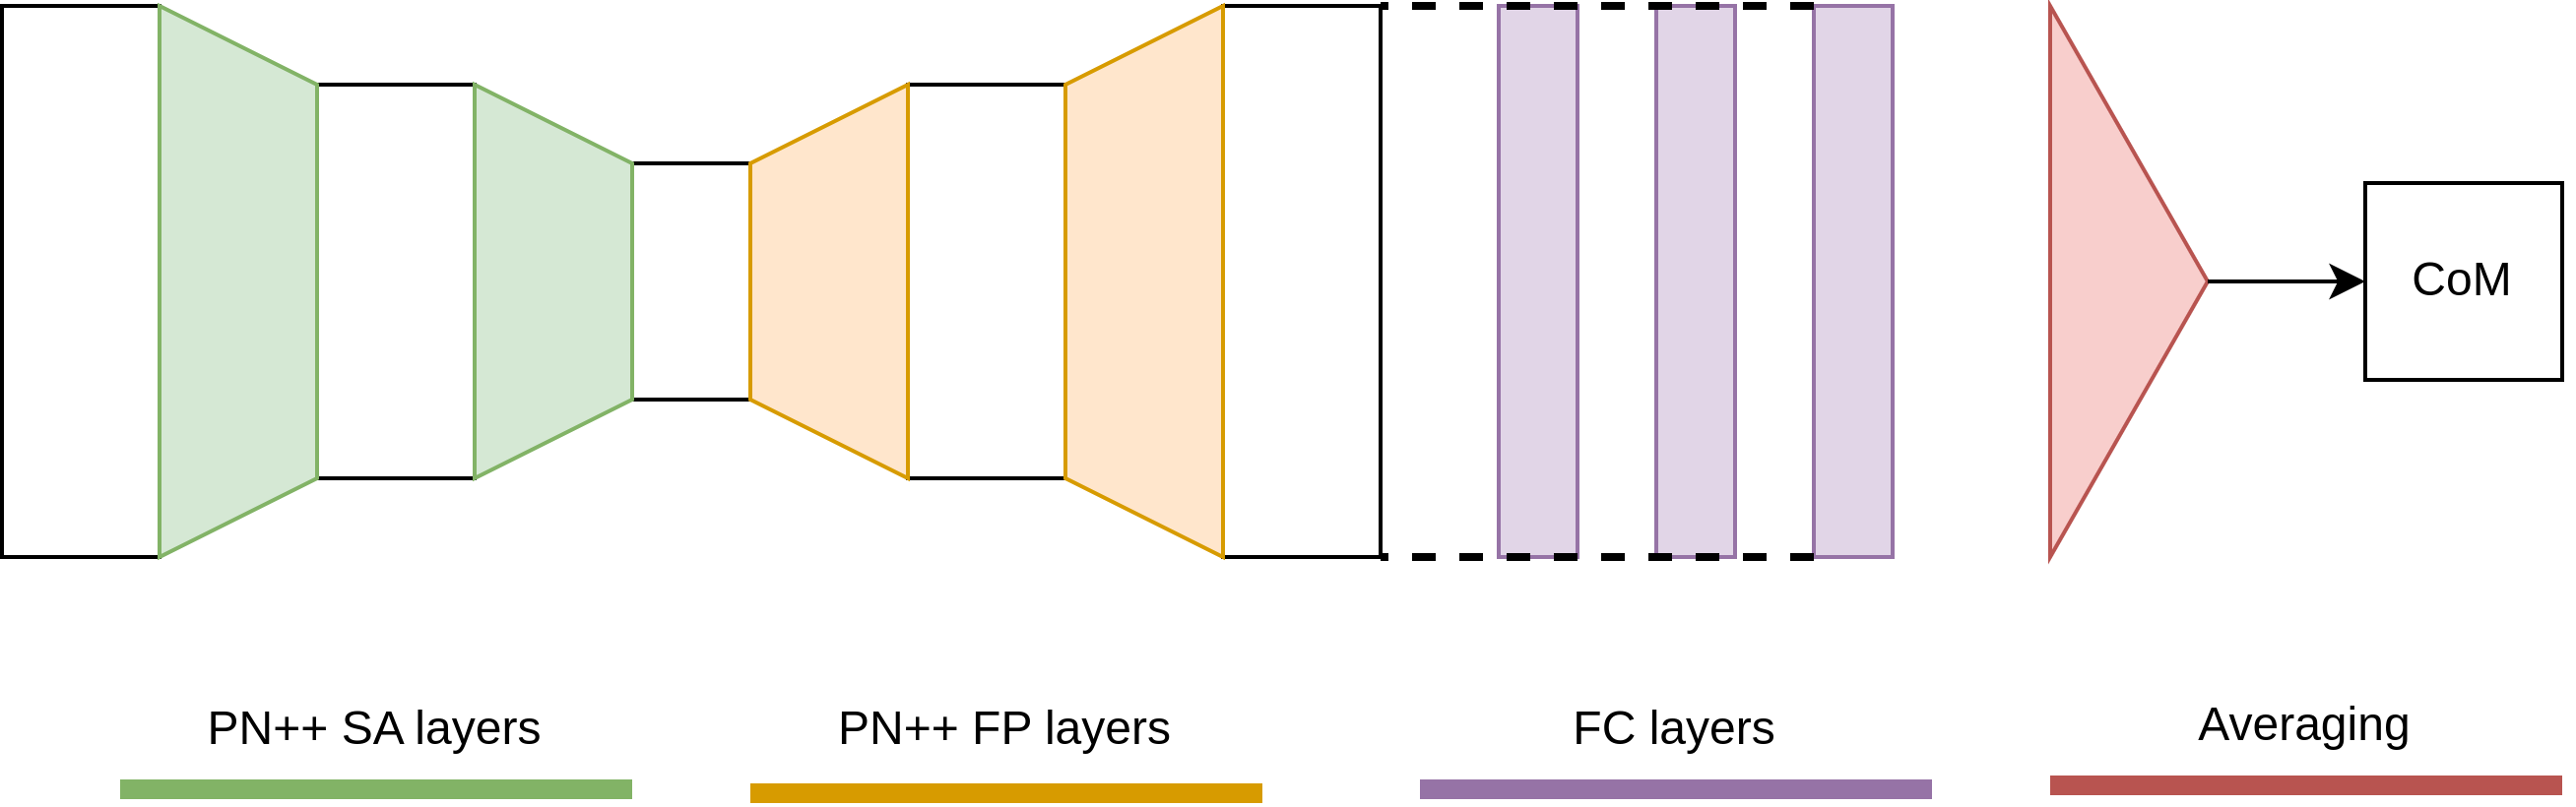
\includegraphics[width=\linewidth]{figures/Architecture.png}
	\caption[Architecture of the center of mass estimator]{The architecture of the center of mass estimator is shown here. The first part of the network is a point cloud feature extractor with three Pointnet++ Set Abstraction layers and three Pointnet++ Feature Propagation layers. The per-point features are then fed into three fully connected layers. As the layers do not reduce in dimensions, they can also be viewed as convolution layers. The fully connected layers produce estimates of the object's center of mass for each point in the}
	\label{fig:architecture}
\end{figure}

\subsection{Point Cloud Augmentation}
The aforementioned architecture achieves a satisfactory performance in terms of overall accuracy. However, there are some egregious failure cases such as predicting CoMs that are below the table \ref{fig:failExample}. To remedy these errors, an "imagined" table point cloud is added similar to \cite{qin2022dexpoint}. In \cite{qin2022dexpoint}, an imaginary hand point cloud is added to improve the model's cognition of the spatial relationship between the hand and the manipulation target. In the case of CoM estimation, the imaginary table surface point cloud serves a similar purpose. It allows the model to get a better sense of the size of the object even under occlusion. It also allows the model to better assess the the placement of the object on the table. Given that the object must be in a stable placement, additional assumptions about the object's distribution of mass can be made to help with center of mass prediction. With the imaginary table surface point cloud added to augment the segmented partial point cloud of the objects, reductions in egregious errors with CoM estimations decreases significantly.

\begin{figure}
	\centering
	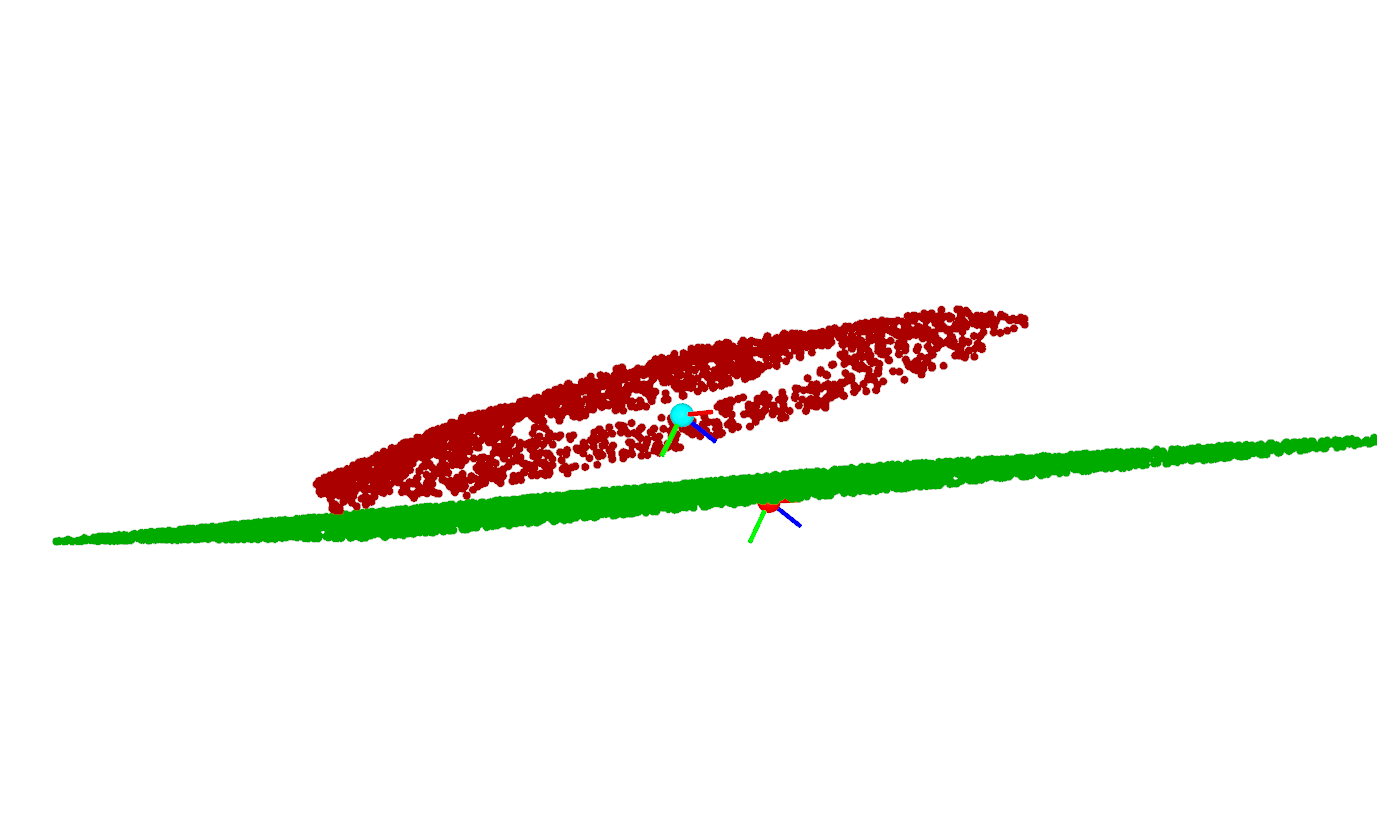
\includegraphics[width=0.6\linewidth]{figures/failExample.png}
	\caption[An example failure with unaugmented point cloud as input]{An example of estimation failure. The ground truth center of mass if shown in blue while the predicted center of mass is shown in red. The object's observed point cloud is shown in red and the table is shown in green. Because only the partial object point cloud is passed to the model, the model is unsure of the exact dimensions of the object and makes a prediction that overestimates the size the object.}
	\label{fig:failExample}
\end{figure}

\subsection{Data Set and Training}
The model is trained using a data set derived from the ACRONYM database \cite{Eppner_Mousavian_Fox_2021}. ACRONYM contains center of mass information of ShapeNet \cite{chang2015shapenet} objects. ACRONYM's toolkit also contains methods that allows the user to generate tabletop scenes. A total of 1000 scenes are generated by placing a random object in a random stable placement on a table. For each scene, five different camera angles that resemble a robot's view of the tabletop are created randomly. Each camera angle would generate a distinct partial point cloud of the object. Each partial point cloud is augmented with a labeled imagined tabletop point cloud; center of mass and a camera matrix annotations are also included. An example of the five point clouds from a different scenes are shown in \ref{fig:PCExamples}.

The model is trained with a learning rate of 0.001 using the ADAM optimizer. The loss function is the average L2 loss of the dense predicted CoM and the ground truth CoM. 

\begin{figure}
	\centering
	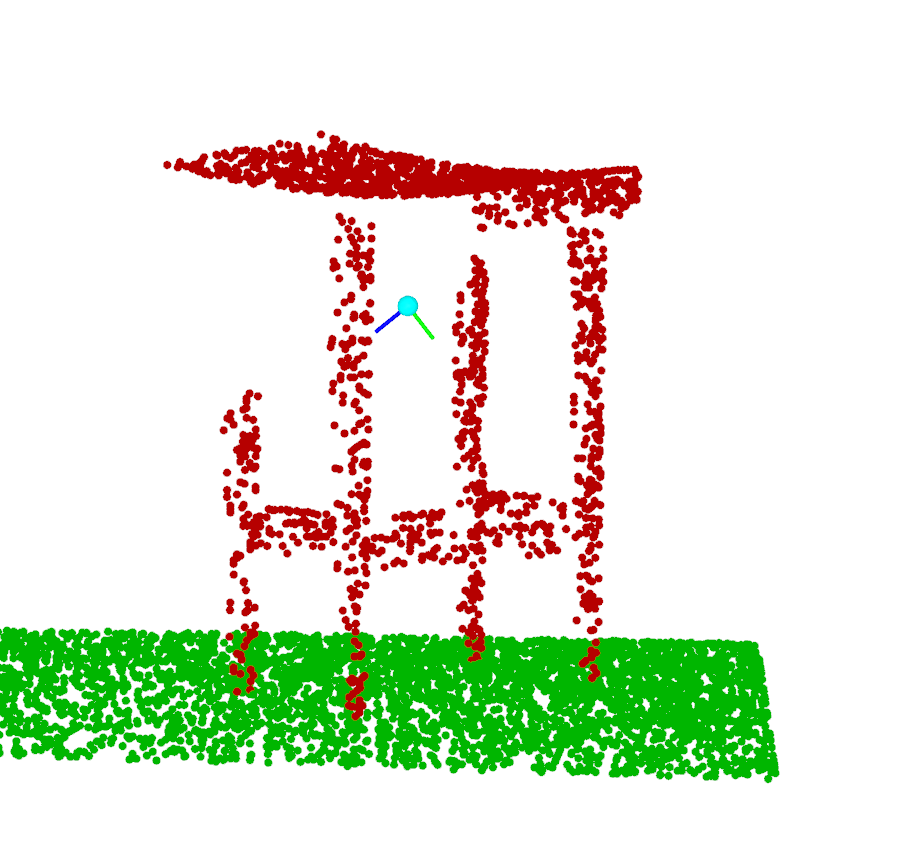
\includegraphics[width=0.19\linewidth]{figures/ex1.png}
	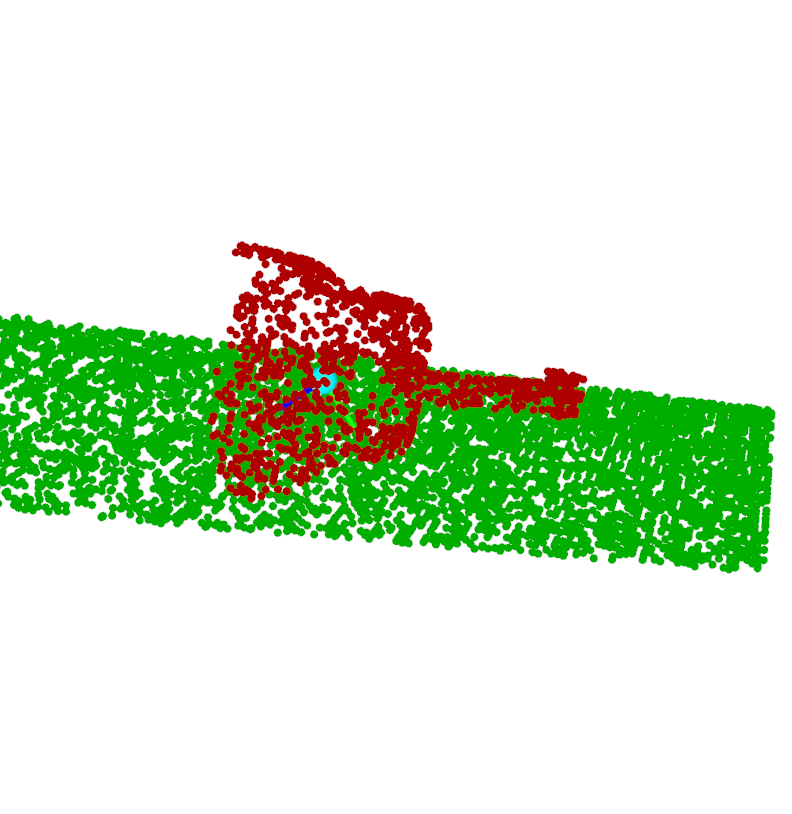
\includegraphics[width=0.19\linewidth]{figures/ex2.png}
	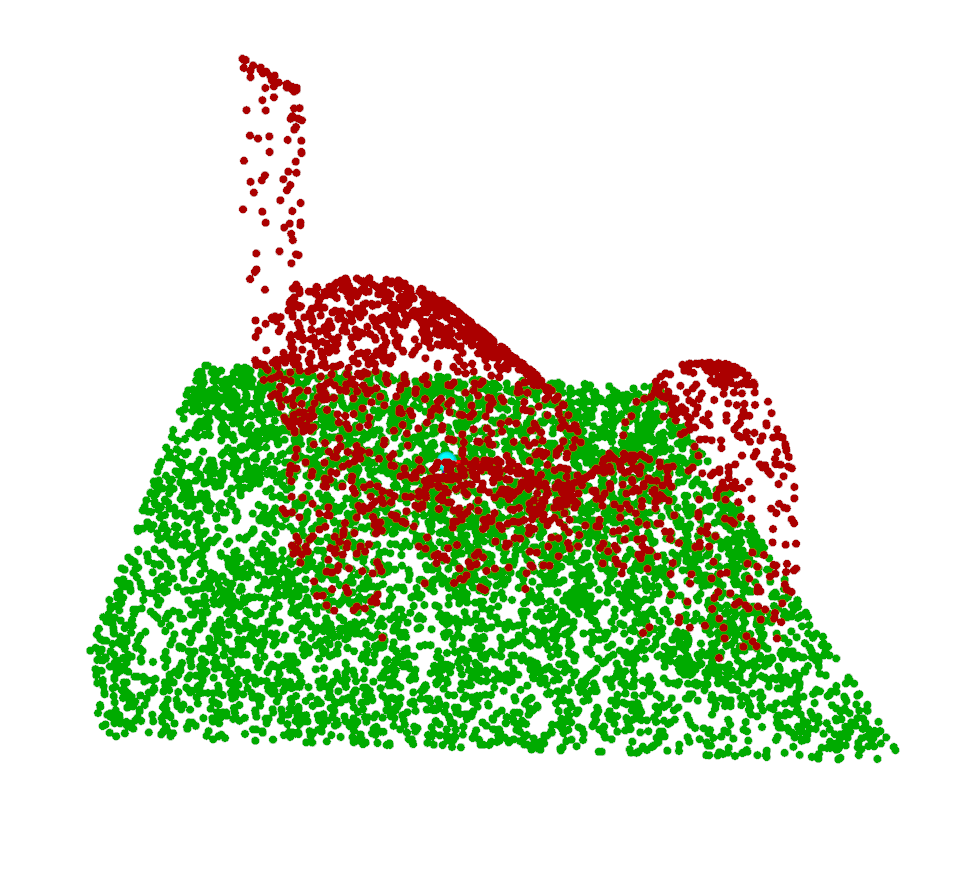
\includegraphics[width=0.19\linewidth]{figures/ex3.png}
	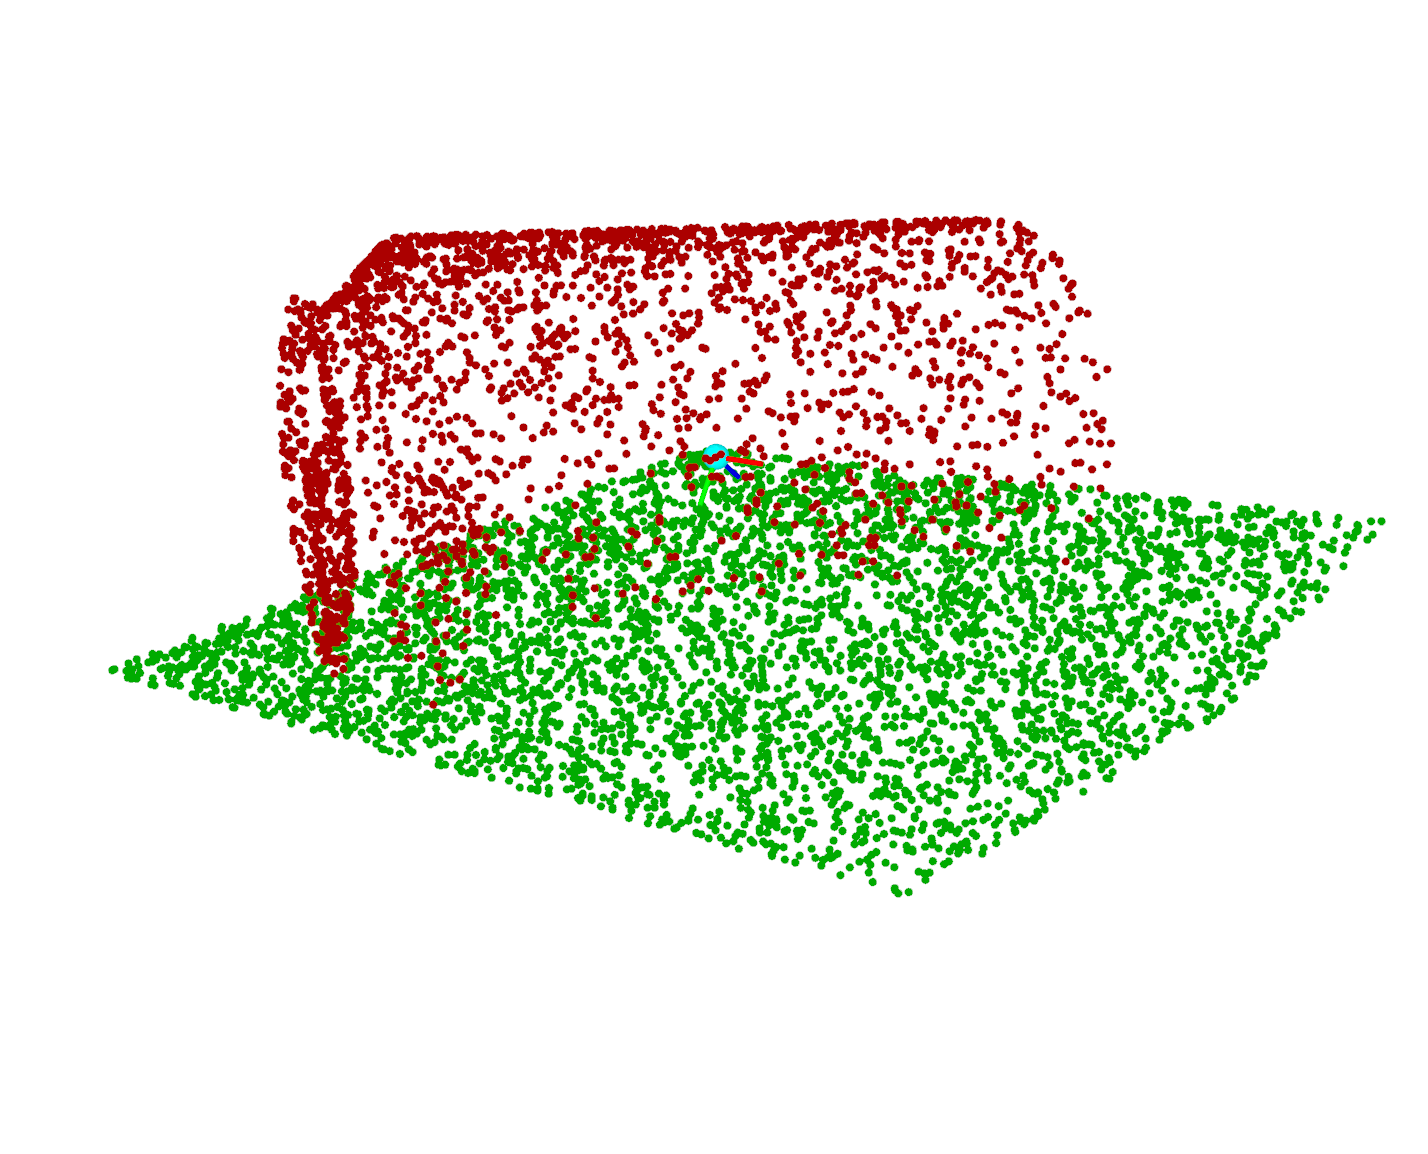
\includegraphics[width=0.19\linewidth]{figures/ex4.png}
	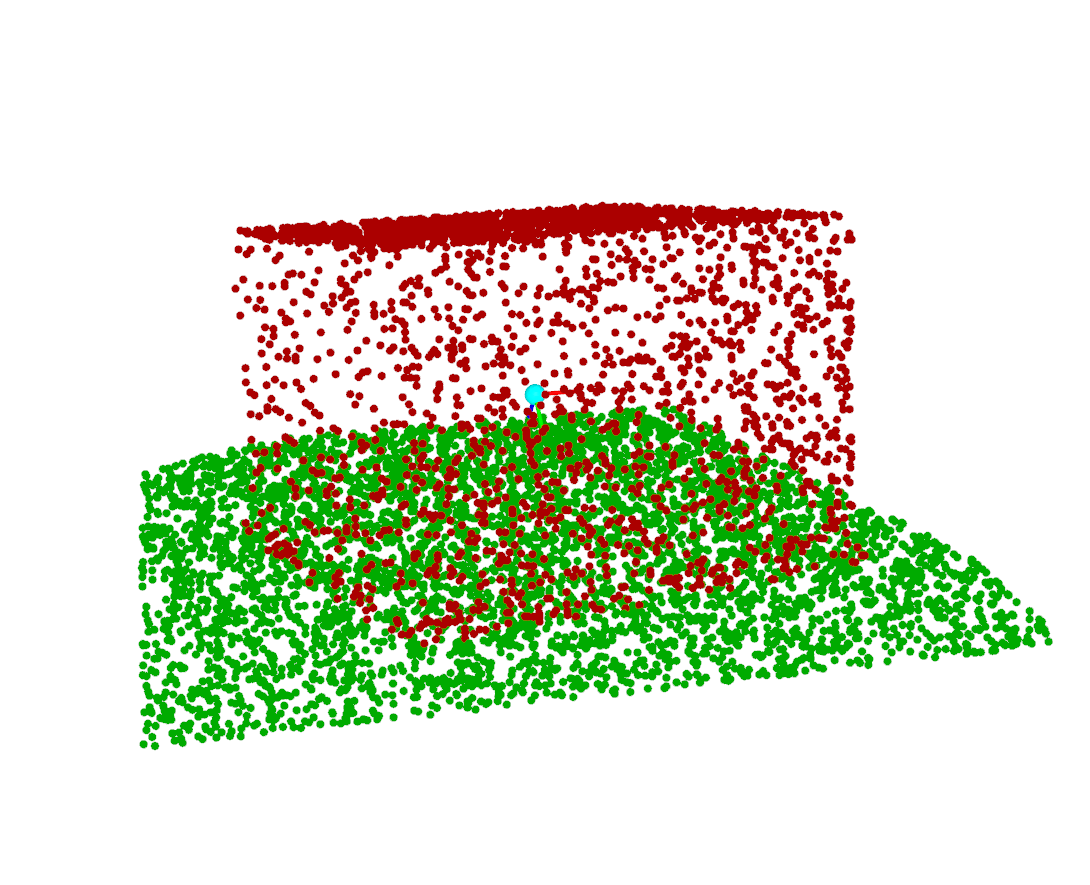
\includegraphics[width=0.19\linewidth]{figures/ex5.png}
	\caption[Example of difference object from different scenes]{Examples of generated data with partial object point cloud in red, augmented table point cloud in green, ground truth center of mass as a blue dot. The axis shown on the ground truth center of mass is aligned with the camera reference frame.}
	\label{fig:PCExamples}
\end{figure}


\section{Grasp Classifier}
The grasp classifier is a torque analyzer tailored to parallel grippers. 


\appendix

% Stuff at the end of the dissertation goes in the back matter
\backmatter
\bibliographystyle{plain} % Or whatever style you want like plainnat
\bibliography{references}

\end{document}
